\subsection{Vito, the UNIPI robot}
\label{sec:vito}

Vito, the UNIPI robot, is the younger brother of Eddie and Boris, the UIBK and UoB robots, respectively. It is a bi-manual robot with a high quality head on top provided by Karlsruhe Institue of Technology. The difference with the other two robots is that Vito uses both Pisa/IIT SoftHands as end-effectors as the default setup. However, its modularity allows him to exchange tools such as a DLR hand, an intrinsic tactile sensors like the one used in DR 3.1, or as an object scanner when using an RGB-D camera and a turntable. Fig.~\ref{fig:vito_gazebo} shows Vito uploaded in the Gazebo environment.

\begin{figure}
\centering
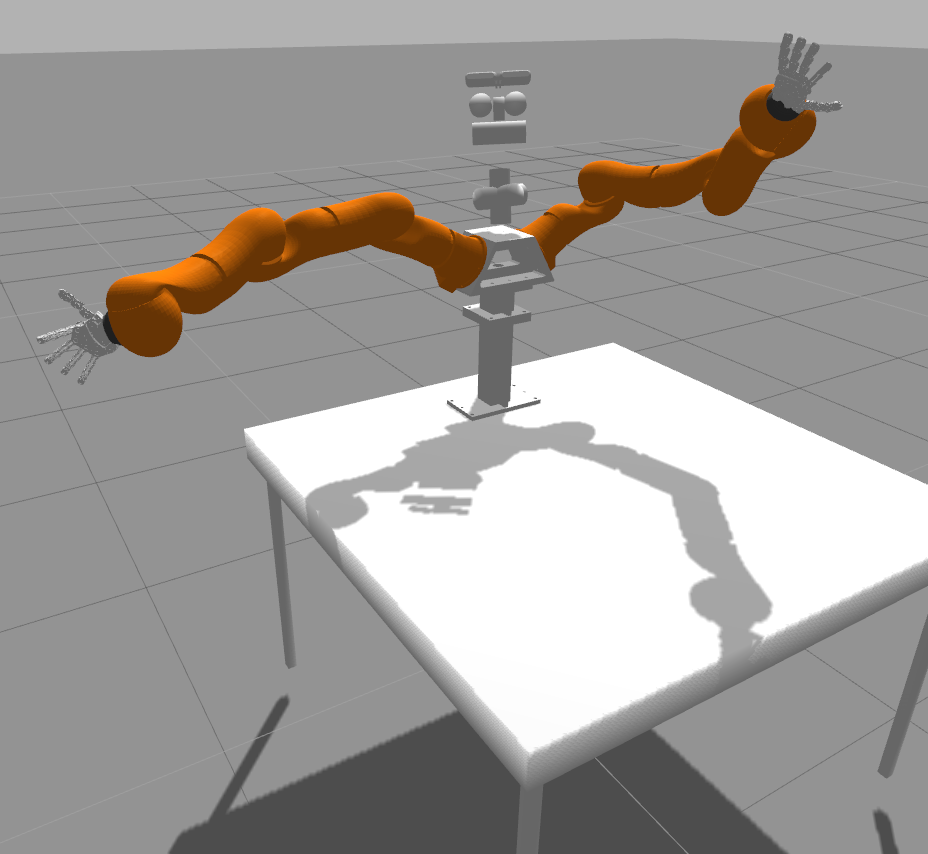
\includegraphics[width=0.7\textwidth]{vito_gazebo.png}
\caption{Vito, the UNIPI robot, in the ROS/Gazebo simulation.}
\label{fig:vito_gazebo}
\end{figure}

\subsubsection{Models and modularity}

All modules, namely arm, hand and head, were developed in such manner that they can be instantiated to create more complex robots like Vito in a very easy and moddular way. In Fig~\ref{fig:vito}, or by clicking \href{https://github.com/CentroEPiaggio/vito_robot/blob/master/vito_description/robot/vito.urdf.xacro}{here}, you can see the actual complete specification of the Vito model. On the top, you see the inclusion of the models, some of them are specific to the robot, such as the torso, table, and couplers, and others are imported such as the arm, hand and head.

\begin{figure}
\tiny
\begin{verbatim}
<?xml version="1.0"?>
<robot xmlns:xacro="http://www.ros.org/wiki/xacro" 
       name="vito">
       
  <!-- MODELS -->
  <xacro:include filename="$(find vito_description)/model/torso.urdf.xacro"/>
  <xacro:include filename="$(find vito_description)/model/table.urdf.xacro"/>
  <xacro:include filename="$(find vito_description)/model/materials.urdf"/>
  <xacro:include filename="$(find vito_description)/model/clamp.urdf.xacro"/>
  <xacro:include filename="$(find vito_description)/model/softhand_base.urdf.xacro"/>
  <xacro:include filename="$(find lwr_description)/model/kuka_lwr.urdf.xacro"/>
  <xacro:include filename="$(find soft_hand_description)/model/soft_hand.urdf.xacro"/>
  <xacro:include filename="$(find kit_head_description)/model/kit_head.urdf.xacro"/>
    
  <link name="world" />
  
  <!-- TABLE -->
  <xacro:model_table name="table" 
                    parent="world"
                    length="1.45"
                    width="1.45"
                    height="0.9"
                    plate_thickness="0.1">
    <origin xyz="-1.22 0.75 0" rpy="0 0 0"/>
  </xacro:model_table>

  <!-- TORSO -->
  <xacro:model_torso name="torso" parent="world">
    <origin xyz="0 0 0"/>
  </xacro:model_torso>
  
  <!-- LEFT ARM -->
  <xacro:kuka_lwr name="left_arm" parent="world">
    <origin xyz="0.0 -0.108585 0.475" 
      rpy="${M_PI*40.8933907/180} ${M_PI*48.5903708/180} ${M_PI*-40.8933907/180}"/>
  </xacro:kuka_lwr>

  <!-- LEFT COUPLERS -->
  <xacro:clamp name="left_clamp" parent="left_arm_7_link">
    <origin xyz="0 0 0.01" rpy="0 0 0"/>
  </xacro:clamp>

  <xacro:softhand_base name="left_base" parent="left_clamp" left="true">
    <origin xyz="0 0 0.004" rpy="0 0 0"/>
  </xacro:softhand_base>

  <!-- LEFT SOFTHAND -->
  <xacro:soft_hand parent="left_base" name="left_hand" left="true" withAdaptiveTransmission="true" useMimicTag="false">
    <origin xyz="0 0 0.0535" rpy="0 0 0"/>
  </xacro:soft_hand>

  <!-- RIGHT ARM -->
  <xacro:kuka_lwr name="right_arm" parent="world">
    <origin xyz="0.0 0.108585 0.475" 
      rpy="${M_PI*-40.8933907/180} ${M_PI*48.5903708/180} ${M_PI*40.8933907/180}"/>
  </xacro:kuka_lwr>

  <!-- RIGHT COUPLERS -->
  <xacro:clamp name="right_clamp" parent="right_arm_7_link">
    <origin xyz="0 0 0.01" rpy="0 0 0"/>
  </xacro:clamp>

  <xacro:softhand_base name="right_base" parent="right_clamp" left="false">
    <origin xyz="0 0 0.004" rpy="0 0 0"/>
  </xacro:softhand_base>

  <!-- RIGHT SOFTHAND -->
  <xacro:soft_hand parent="right_base" name="right_hand" left="false" withAdaptiveTransmission="true" useMimicTag="false">
    <origin xyz="0 0 0.0535" rpy="0 0 0"/>
  </xacro:soft_hand>

  <!-- HEAD -->
  <xacro:kit_head name="head" parent="world">
    <origin xyz="0.0 0.0 ${0.55 + 0.1}" rpy="0.0 0.0 3.141592"/>
  </xacro:kit_head>

</robot>
\end{verbatim}
\caption{Vito definition using the available models as components, namely the arm, hand and head.}
\label{fig:vito}
\end{figure}


\subsubsection{Real/Simulation planning and control framework}

The planning framework is heavily based on the MoveIt! package, since motion planning is not within the goals of the project. It is worth to mention that Section ``High-Level Planning for Dual Arm Goal-Oriented Task'' in DR 4.2 interfaces with the core planning functions of the package to generate and use the transition graph.

For the control framework, each module implements an interface to the real or the simulated hardware, looking for maximum similarities between the two scenarios to have a switch between reality and simulation as effortless as possible. Both hardware interfaces expose the joints as resources that can be controlled using effort, position, or even velocity commands. This depends on the available hardware. Moreover, controllers that are compatible with the resources exposed by the hardware interface can be used indistinctly. All controllers are gathered in a configuration file that defines its functional parameters, such as the proportional, derivative and integral gains in a PID controller. Such controllers are listed as the way a group of joints can be moved in a regulated way to execute trajectories, perform exploration, or move to any desired position in the workspace. Given the fact that the main PaCMan contribution is not on trajectory planning, we decided to use the MoveIt! library to tackle this aspect.

The plan-to-action framework can be summarized in Fig.~\ref{fig:framework}. The link between the two figures is the controllers, in the sense that they must understand the planning output, typically joint trajectories, and the commanded values must be compatible with the hardware resource types, typically position and effort commands.

\begin{figure}
\centering
\begin{subfigure}[t]{0.58\textwidth}
\centerline{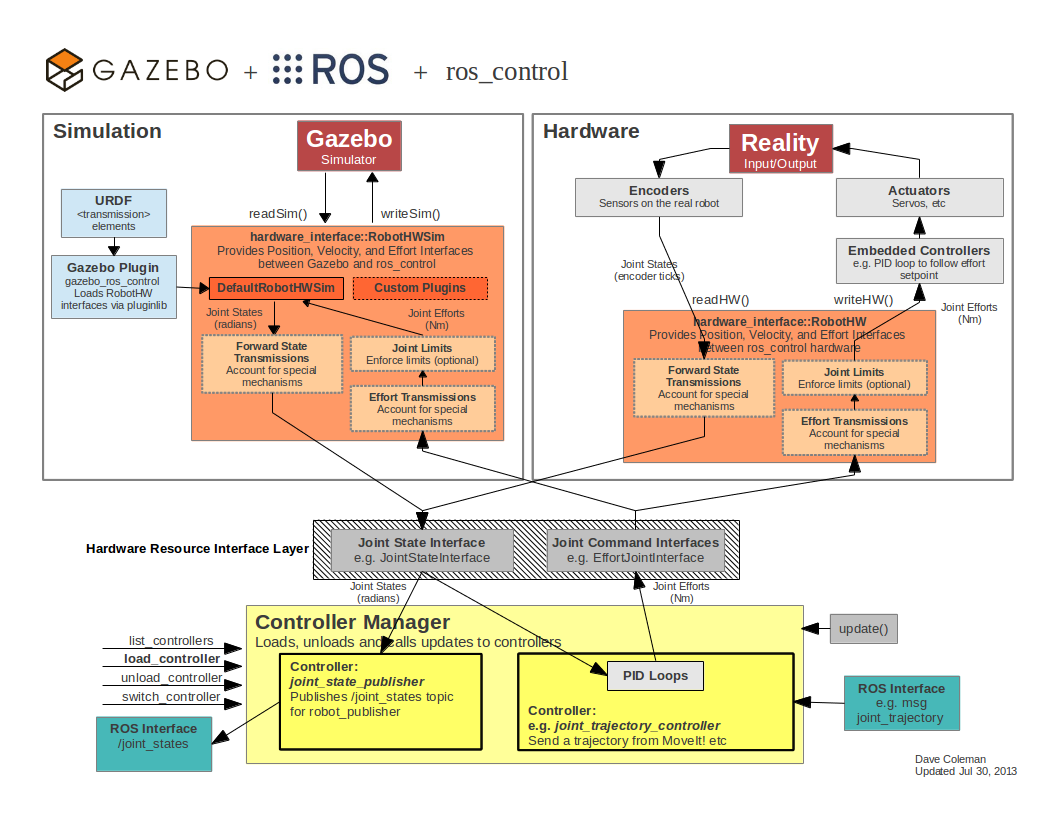
\includegraphics[width=\textwidth]{ros+gazebo.png}}
\caption{ROS/Gazebo framework.}
\label{fig:rosgazebointeraction}
\end{subfigure}
\begin{subfigure}[t]{0.4\textwidth}
\centerline{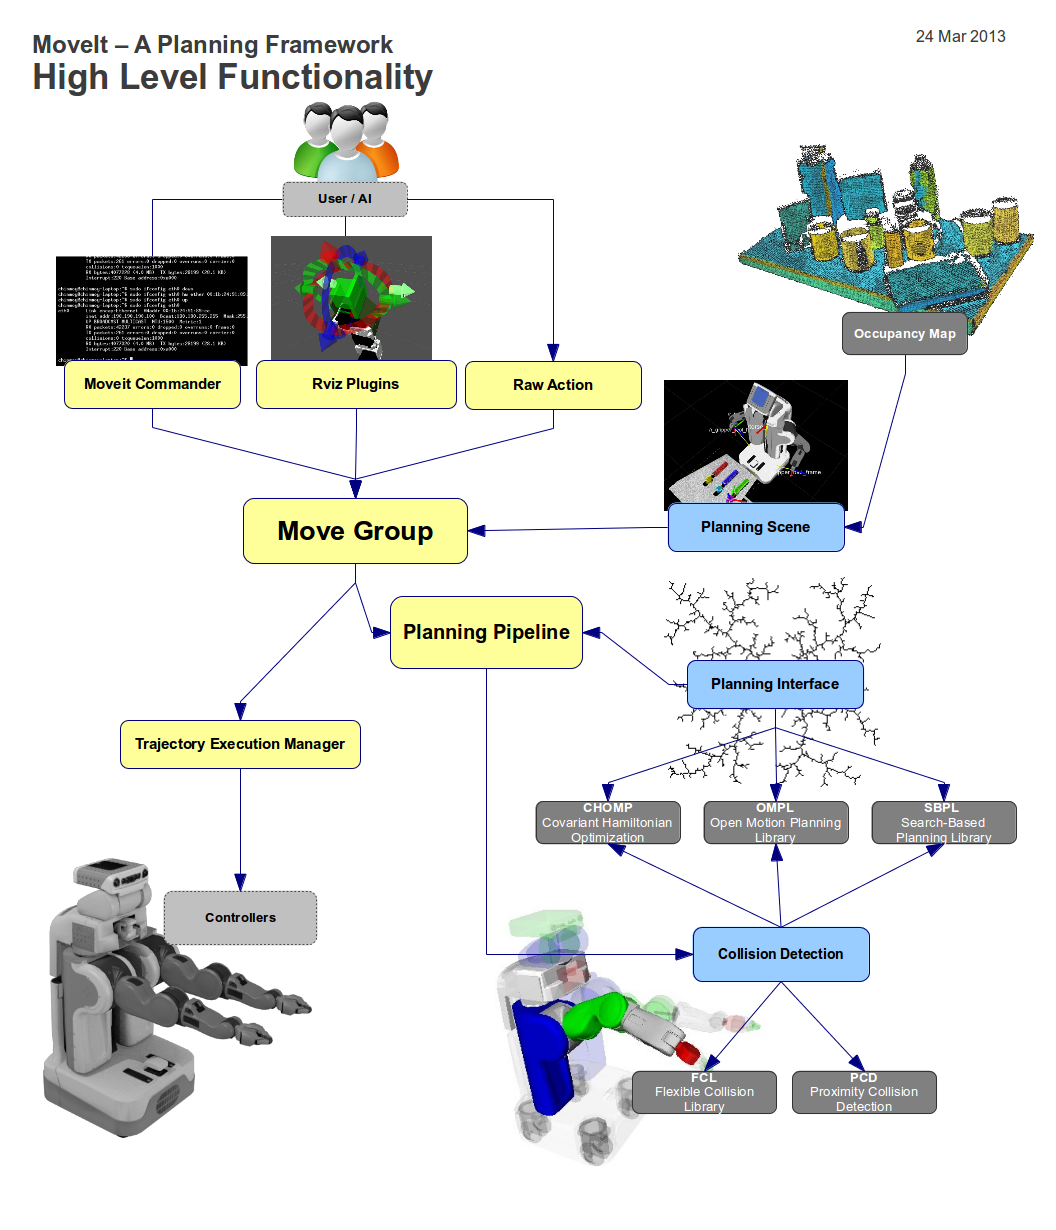
\includegraphics[width=\textwidth]{moveit_highlevel.png}}
\caption{MoveIt! framework.}
\label{fig:planning}
\end{subfigure}
\caption{Real/Simulation planning and control framework}
\label{fig:framework}
\end{figure}

Particularly, the arm~(see Sec.~\ref{sec:kuka}) works with both effort and position using the same hardware interface in both real and simulation, and the hand (see Sec.~\ref{sec:softhand}) and head~(see Sec.~\ref{sec:kithead}) offer only position controlled motors. Next, we describe more details on the hardware interface of each module. In the case of the arm, special attention is given to the implementation of additional controllers that make the most of the arm capabilities for the required tasks within the project. In the case of the hand, special attention is given to the implementation of the adaptive synergy transmission to replicate in simulation the adaptivity the hand has in reality.
%With this in mind, the planning and execution phase  at a robust object exploration and grasping.